
\documentclass{report}
% alternatives: scrartcl, article or report


%%%%% PACKAGES

% small tweaks and nicer typography
\usepackage{microtype}
\usepackage{hyperref}

% dealing with figures
\usepackage{subcaption}
\usepackage{wrapfig}

% basic math stuff
\usepackage{mathtools}
\usepackage{amssymb}
\usepackage{amsthm}
%\usepackage{tikz-cd}
\usepackage{cancel}
\usepackage{cases}
\usepackage{dsfont}

% tikz
\usepackage{tikz}
\usepackage{pgfplots}
\usetikzlibrary{positioning}
%\usetikzlibrary{patterns}
%\usetikzlibrary{babel}
\tikzset{>=stealth}
\usepackage{wrapfig}

% code
\usepackage{listings}
\usepackage{pythonhighlight}

%%%% Graphics %%%%%

%\graphicspath{{Plots/}}

%\newcommand{\tikzmark}[3][]{\tikz[remember picture,baseline] \node [anchor=base,#1](#2) {$#3$};}

%\usepackage{booktabs}
%\usepackage{bm}
%\usepackage{minted}

% for inkscape images
%\usepackage{pdftricks}
%\begin{psinputs}
%   \usepackage{pstricks}
%   \usepackage{multido}
%\end{psinputs}
%\usepackage[pdf]{pstricks}
%\usepackage{import}


\usepackage[backend=bibtex]{biblatex}
\addbibresource{mybib.bib}


%%%%% CONFIGURATION

% prevents automatic line breaks inside of equations
% since it looks bad
\binoppenalty = \maxdimen
\relpenalty   = \maxdimen

% theorem-like environments
\newcounter{everything}
\newtheorem{corollary}[everything]{Corollary}
\newtheorem{lemma}[everything]{Lemma}
\newtheorem{proposition}[everything]{Proposition}
\newtheorem{theorem}[everything]{Theorem}
\newtheorem*{claim}{Claim}
\newtheorem*{given}{Given}


%%%%% CUSTOM COMMANDS

% real numbers via \R
% complex numbers via \C
% general field via \K
\def\C{\mathbb{C}}
\def\R{\mathbb{R}}
\def\K{\mathbb{K}}
\def\Q{\mathbb{Q}}
\def\Z{\mathbb{Z}}
\def\N{\mathbb{N}}
\def\H{\mathbb{H}}
\def\e{\varepsilon}

\newcommand{\cA}{\mathcal{A}}
\newcommand{\cB}{\mathcal{B}}
\newcommand{\cC}{\mathcal{C}}
\newcommand{\cD}{\mathcal{D}}
\newcommand{\cE}{\mathcal{E}}
\newcommand{\cF}{\mathcal{F}}
\newcommand{\cG}{\mathcal{G}}
\newcommand{\cH}{\mathcal{H}}
\newcommand{\cI}{\mathcal{I}}
\newcommand{\cJ}{\mathcal{J}}
\newcommand{\cK}{\mathcal{K}}
\newcommand{\cL}{\mathcal{L}}
\newcommand{\cM}{\mathcal{M}}
\newcommand{\cN}{\mathcal{N}}
\newcommand{\cO}{\mathcal{O}}
\newcommand{\cP}{\mathcal{P}}
\newcommand{\cQ}{\mathcal{Q}}
\newcommand{\cR}{\mathcal{R}}
\newcommand{\cS}{\mathcal{S}}
\newcommand{\cT}{\mathcal{T}}
\newcommand{\cU}{\mathcal{U}}
\newcommand{\cV}{\mathcal{V}}
\newcommand{\cW}{\mathcal{W}}
\newcommand{\cX}{\mathcal{X}}
\newcommand{\cY}{\mathcal{Y}}
\newcommand{\cZ}{\mathcal{Z}}

\newcommand{\bA}{\mathbb{A}}
\newcommand{\bB}{\mathbb{B}}
\newcommand{\bC}{\mathbb{C}}
\newcommand{\bD}{\mathbb{D}}
\newcommand{\bE}{\mathbb{E}}
\newcommand{\bF}{\mathbb{F}}
\newcommand{\bG}{\mathbb{G}}
\newcommand{\bH}{\mathbb{H}}
\newcommand{\bI}{\mathbb{I}}
\newcommand{\bJ}{\mathbb{J}}
\newcommand{\bK}{\mathbb{K}}
\newcommand{\bL}{\mathbb{L}}
\newcommand{\bM}{\mathbb{M}}
\newcommand{\bN}{\mathbb{N}}
\newcommand{\bO}{\mathbb{O}}
\newcommand{\bP}{\mathbb{P}}
\newcommand{\bQ}{\mathbb{Q}}
\newcommand{\bR}{\mathbb{R}}
\newcommand{\bS}{\mathbb{S}}
\newcommand{\bT}{\mathbb{T}}
\newcommand{\bU}{\mathbb{U}}
\newcommand{\bV}{\mathbb{V}}
\newcommand{\bW}{\mathbb{W}}
\newcommand{\bX}{\mathbb{X}}
\newcommand{\bY}{\mathbb{Y}}
\newcommand{\bZ}{\mathbb{Z}}

\newcommand{\dif}[1]{\,\mathrm{d} #1}
%\newcommand{\norm}[1]{\lVert #1 \rVert}
%\newcommand{\abs}[1]{\left| #1 \right|}
\newcommand{\bnorm}[1]{\left\lVert #1\right\rVert}
\newcommand{\vii}[2]{\ensuremath{\begin{bmatrix}#1 \\ #2 \end{bmatrix}}}
\newcommand{\mii}[4]{\ensuremath{\begin{bmatrix}#1&#2 \\ #3&#4 \end{bmatrix}}}
\newcommand{\mc}[1]{\mathcal{#1}}

\newcommand{\one}{\mathds{1}}
\newcommand{\bigO}{\mathcal{O}}


%%%%%%%%%%    Math operators    %%%%%%%%%%%%%%%%%%%%%%%%%%%

\DeclareMathOperator{\Id}{Id}             % identity morphism
% \DeclareMathOperator{\ker}{ker}           % kernel
\DeclareMathOperator{\rg}{rg}             % image
\DeclareMathOperator{\defekt}{def}             % defect
\DeclareMathOperator{\im}{im}             % image
\DeclareMathOperator{\Hom}{Hom}           % homomorphisms
\DeclareMathOperator{\End}{End}           % endomorphisms
\DeclareMathOperator{\Span}{Span}         % linear span
\DeclareMathOperator{\grad}{\nabla}         % gradient
\DeclareMathOperator{\diam}{diam}         % gradient
\DeclareMathOperator{\Tr}{Tr}       	  % trace
\DeclareMathOperator{\diver}{Div}			% divergence
\DeclareMathOperator{\supp}{supp}			% support
\DeclareMathOperator{\dist}{dist}			% distance
\DeclareMathOperator{\inter}{int}			% interiour
\DeclareMathOperator{\epi}{epi}			% epigraph
\DeclareMathOperator{\hyp}{hyp}			% hypograph
\DeclareMathOperator{\Lip}{Lip}			% lipschitz konstant
\DeclareMathOperator{\graph}{graph}			% graph
\DeclareMathOperator{\sgn}{sgn}			% sign
\DeclareMathOperator{\BMO}{BMO}			% BMO
\DeclareMathOperator{\mean}{mean}			% BMO
%\DeclareMathOperator{\B}{B}			% BMO

% inner product (scalar product) via \inner{v, w}
% norm via \norm{x}
% absolute value via \abs{x}
% use the star-version for automatic scaling
\DeclarePairedDelimiter{\abs}{\lvert}{\rvert}
\DeclarePairedDelimiter{\inner}{\langle}{\rangle}
\DeclarePairedDelimiter{\norm}{\lVert}{\rVert}

% \vect{ x // y // z } for a column vector with entries x, y, z
% similarly for larger vectors
% in this code:  1 = number of arguments
%               #1 = first argument
\newcommand{\vect}[1]{\begin{bmatrix} #1 \end{bmatrix}}
\newcommand{\commentops}[2]{\stackrel{\mathclap{#1}}{#2}}


% \conj{z} for complex conjugation
\newcommand{\conj}{\overline}

%counter of current constant number:    
\newcounter{constant} 
%defines a new constant, but does not typeset anything:
\newcommand{\newconstant}[1]{\refstepcounter{constant}\label{#1}} 
%typesets named constant:
\newcommand{\useconstant}[1]{c_{\ref{#1}}}

%%%%%%% GENERAL STYLE %%%%%%%%%%%%%%%%%%

%\setcounter{tocdepth}{3}


%%%%% TITLE PAGE

%\subject{Simulation Tools, VT23}
\title{Project Reports}
\author{Salvador Castagnino, Theo Koppenhöfer}
\date{\today}


%%%%% The content starts here %%%%%%%%%%%%%


\begin{document}

\maketitle

\chapter*{Project 1}

\section*{Introduction}

\subsection*{The Benchmark}

In the following we use the model of a pendulum attached to a rod which is elastic in the radial direction as described in Task 1. The situation is depicted in figure \ref{dr:Pendulum}.

\begin{wrapfigure}{r}{0.43\textwidth}
\centering
\input{../Drawings/pendulum.pdf_tex}
\caption{The pendulum}
\label{dr:Pendulum}
\end{wrapfigure}

This problem leads to the formulation as an ODE
\begin{align*}
	\vect{y_1 \\ y_2 \\ y_3 \\ y_4}' = \vect{y_3 \\ y_4 \\ -y_1\lambda(y_1,y_2) \\ -y_2\lambda(y_1,y_2)-1}
\end{align*}
with
\begin{align*}
	\lambda(y_1,y_2)=k\frac{\norm{(y_1,y_2)}-1}{\norm{(y_1,y_2)}}\,.
\end{align*}
The plot of a numerical solution to this problem for $k=1$ can be seen in figures \ref{pl:StateTime1} \ref{pl:PhasePortrait1} and \ref{pl:PolarPlot1}.

\begin{figure}[h]
\centering
\begin{minipage}[b]{0.45\textwidth}
\centering
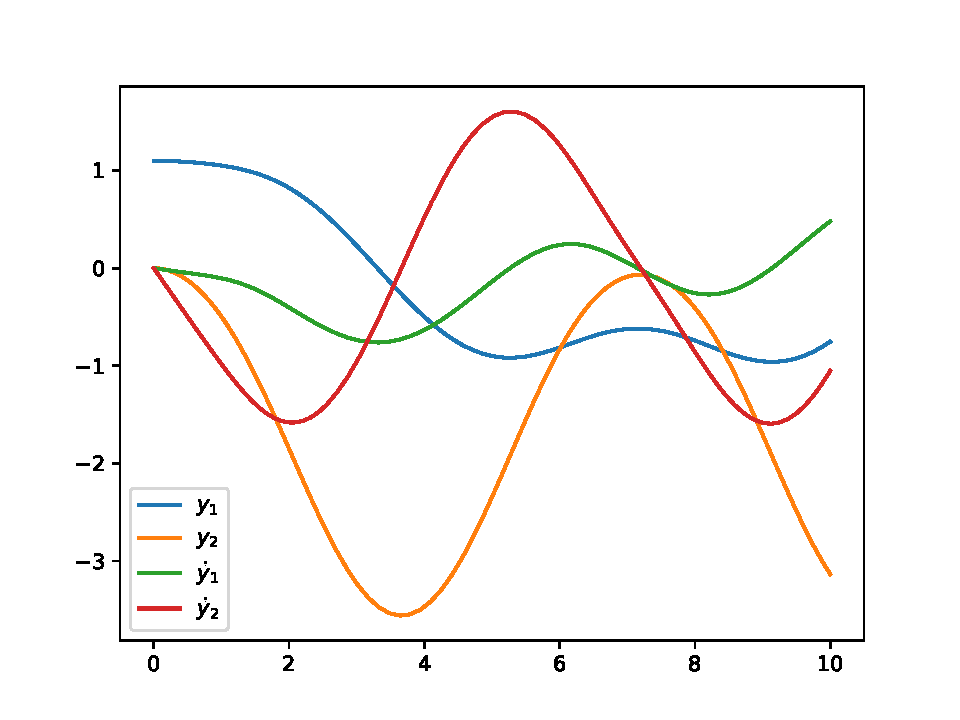
\includegraphics[width=\textwidth]{../Plots/Task4/Figure_1}
\caption{State in dependence of time.}
\label{pl:StateTime1}
\end{minipage}
\hfill
\begin{minipage}[b]{0.45\textwidth}
\centering
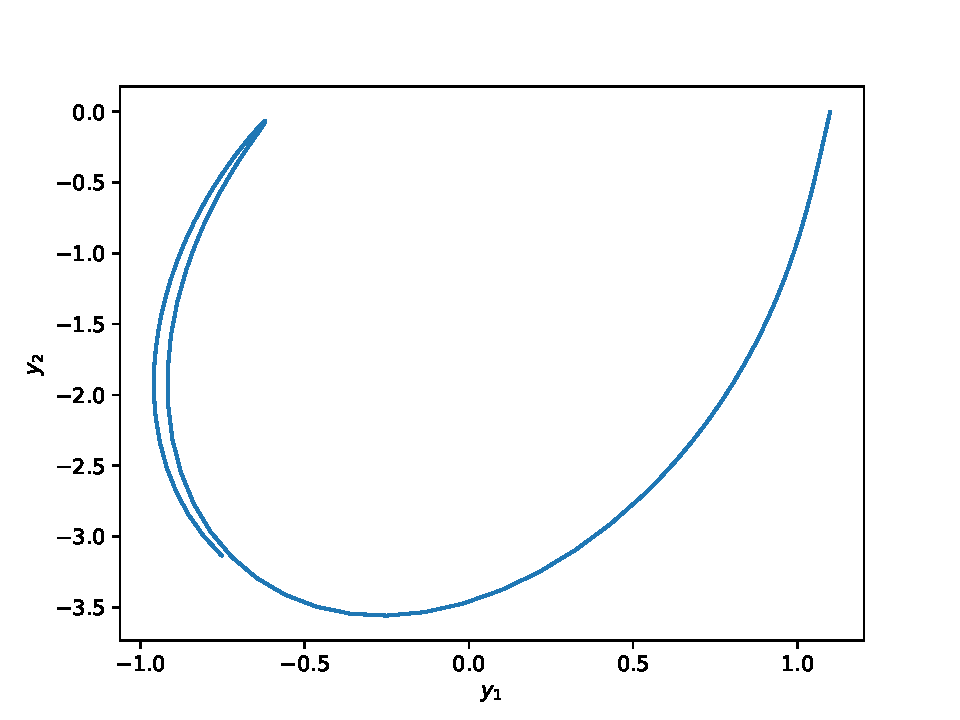
\includegraphics[width=\textwidth]{../Plots/Task4/Figure_2}
\caption{Path traced out by pendulum.}
\label{pl:PhasePortrait1}
\end{minipage}
\end{figure}

We can calculate the potential, kinetic and approximate the elastic energy with the formulas
\begin{align*}
	E_{\text{pot}}=1+y_2
	\qquad\qquad E_{\text{kin}}=\frac{\norm{(y_3,y_4)}^2}{2}
	\qquad\qquad E_{\text{elast}}=k\frac{(\norm{(y_1,y_2)}-1)^2}{2}\,.
\end{align*}
Adding these up we get the approximate total energy
\begin{align*}
	E_{\text{tot}}=E_{\text{pot}}+E_{\text{kin}}+E_{\text{elast}}\,.
\end{align*}
We expect the approximate total energy to be constant which indeed can be seen in Figure \ref{pl:EnergyPlot1} for that previously calculated numerical solution.
Because of this property we can use the relative variation of the approximate total energy as an index to measure the stability of the method. We specifically implement
\begin{python}
import numpy as np
instability_index = (np.max(total_energy)-np.min(total_energy)) \
				              /np.mean(total_energy)
\end{python}
In the ideal world this index almost vanishes.

\begin{figure}[h]
\centering
\begin{minipage}[b]{0.45\textwidth}
\centering
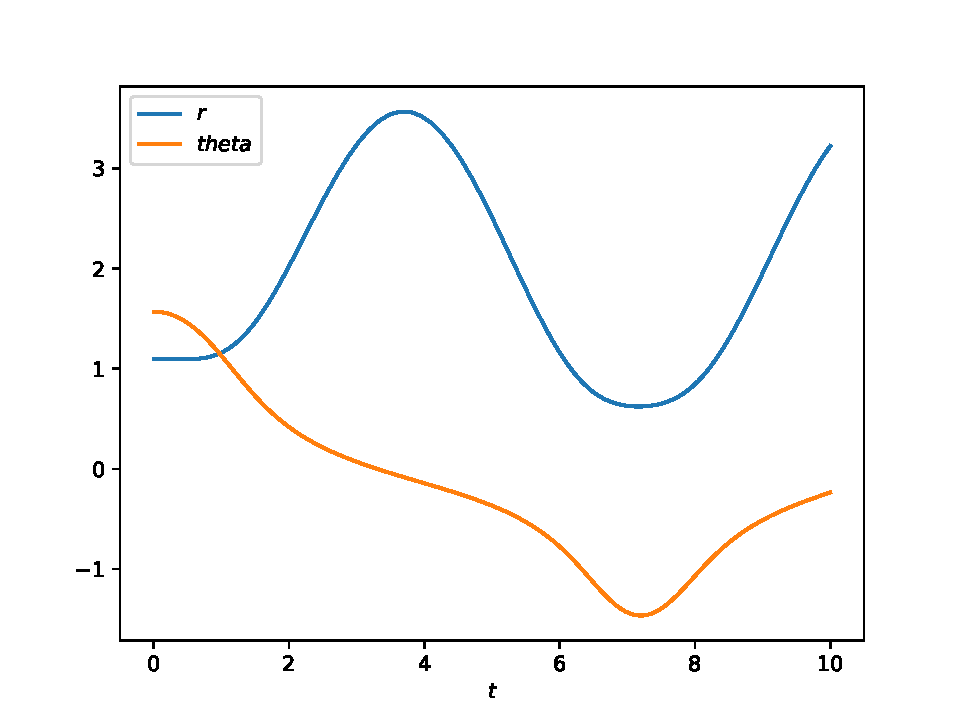
\includegraphics[width=\textwidth]{../Plots/Task4/Figure_0}
\caption{Polar coordinates.}
\label{pl:PolarPlot1}
\end{minipage}
\hfill
\begin{minipage}[b]{0.45\textwidth}
\centering
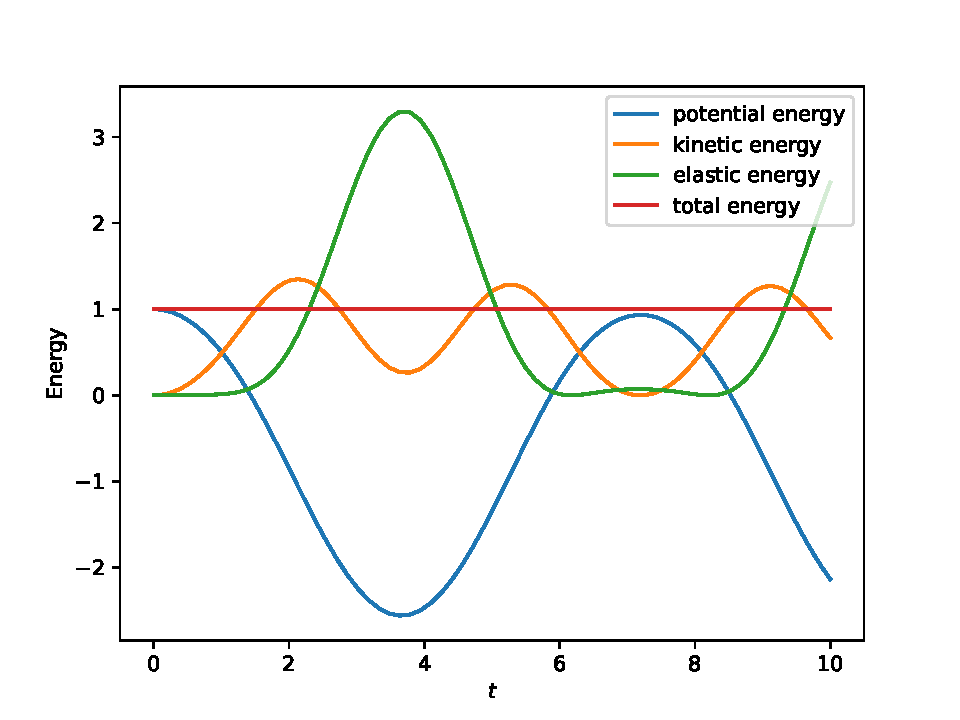
\includegraphics[width=\textwidth]{../Plots/Task4/Figure_3}
\caption{Energy plot}
\label{pl:EnergyPlot1}
\end{minipage}
\end{figure}

\section*{Testing Explicit Methods}

For linear problems, explicit methods present a much reduced stability region which dictates the possible step sizes for that specific method.
For the problem of the elastic pendulum, approximated by explicit methods, when the value of $k$ is increased we are expected to see the approximation blow up showing oscillations of unbounded amplitude.
This unstable behavior will be attenuated by reducing the value of the step $h$.

The problem was simulated using Explicit Euler and RK4.
All the experiments in this section, if not otherwise stated, take as initial value $y_0 = [1.1, 0, 0, 0]$ and have $[0, 20]$ for domain.
The graphs are presented in polar coordinates where $r$ refers to the length of the spring and $\theta$ refers to the angle conformed between the pendulum and the vertical axis.

It can be observed that for a step size of $h=0.01$ Explicit Eurler (Figure \ref{exp_euler_k=50_h=0.01_c}) already shows instability for values of $k=50$ while RK4 (Figure \ref{rk4_h=0.01_k=3000_c}) with that same step size remains stable for values up to $k=3000$.

\begin{figure}[h]
\centering
\begin{minipage}[b]{0.45\textwidth}
\centering
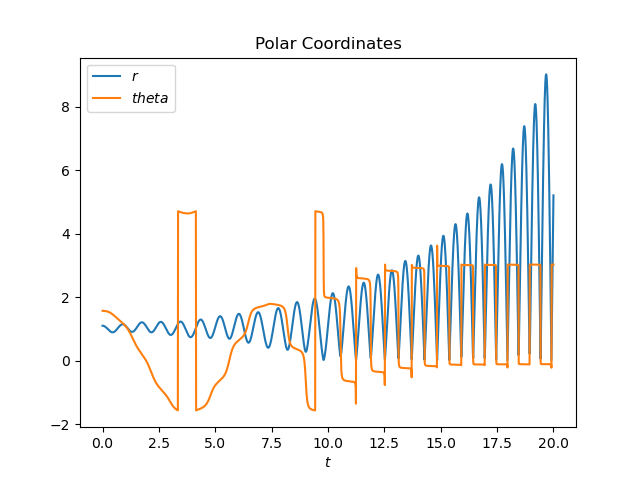
\includegraphics[width=\textwidth]{../Plots/ExpEuler/exp_euler_k=50_h=0.01_c}
\caption{Explicit Euler $h=0.01$ $k=50$}
\label{exp_euler_k=50_h=0.01_c}
\end{minipage}
\hfill
\begin{minipage}[b]{0.45\textwidth}
\centering
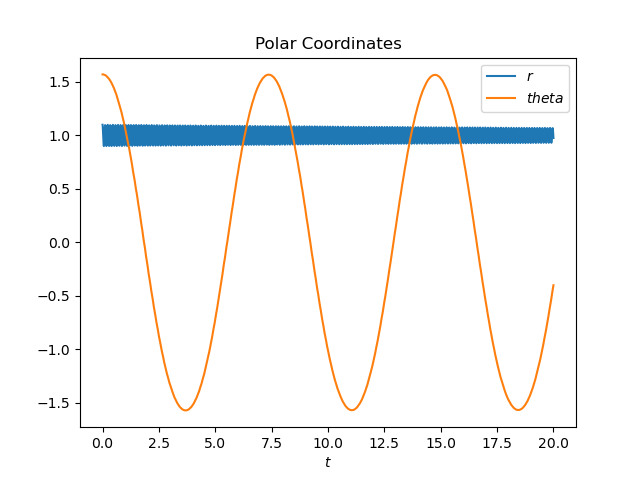
\includegraphics[width=\textwidth]{../Plots/RK4/rk4_h=0.01_k=3000_c}
\caption{RK4 $h=0.01$ $k=3000$}
\label{rk4_h=0.01_k=3000_c}
\end{minipage}
\end{figure}
	
For Explicit Euler (Figure \ref{exp_euler_k=50_h=0.001_c_2}), by keeping the value of $k$ constant and reducing the step size by a decimal place we can see how the instability is attenuated presenting a similar amplitude over time.
It takes a much larger step size and spring constant for RK4 to become unstable (Figure \ref{rk4_h=0.1_k=975_c}), once unstabilized it’s growth is much more rapid than Explicit Euler’s and it does so without oscillating.

\begin{figure}[h]
\centering
\begin{minipage}[b]{0.45\textwidth}
\centering
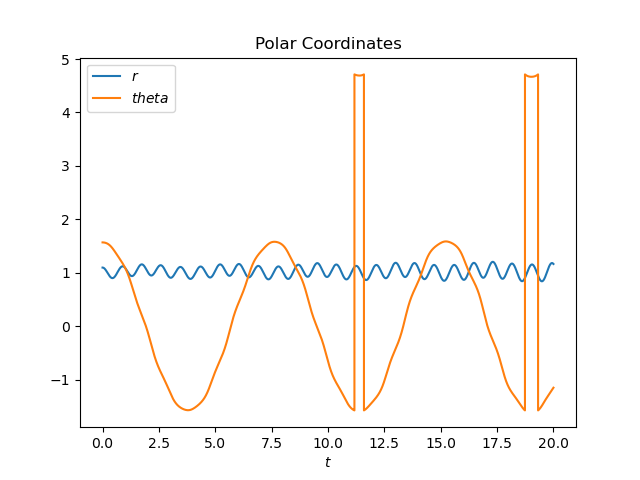
\includegraphics[width=\textwidth]{../Plots/ExpEuler/exp_euler_k=50_h=0.001_c}
\caption{Explicit Euler $h=0.001$ $k=50$}
\label{exp_euler_k=50_h=0.001_c_2}
\end{minipage}
\hfill
\begin{minipage}[b]{0.45\textwidth}
\centering
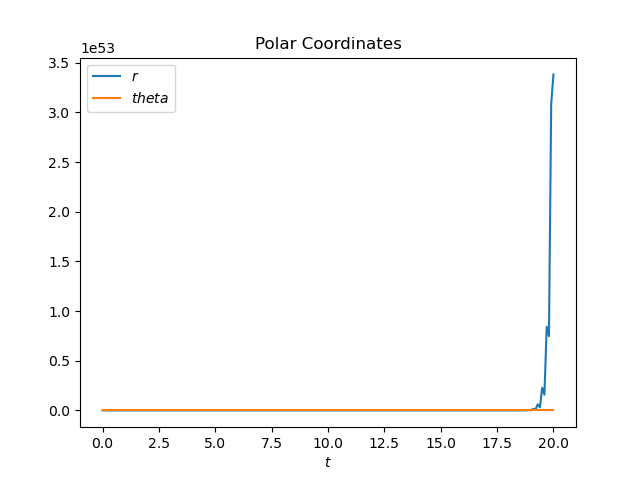
\includegraphics[width=\textwidth]{../Plots/RK4/rk4_h=0.1_k=975_c}
\caption{RK4 $h=0.1$ $k=975$}
\label{rk4_h=0.1_k=975_c}
\end{minipage}
\end{figure}

It is interesting to observe that the oscillation of the spring is rapidly dumped when using RK4 (Figure \ref{rk4_h=0.1_k=300_c}), a behavior similar to that presented by implicit methods.
This behavior cannot be observed in the other explicit methods.

\begin{figure}[h]
\centering
\begin{minipage}[b]{0.45\textwidth}
\centering
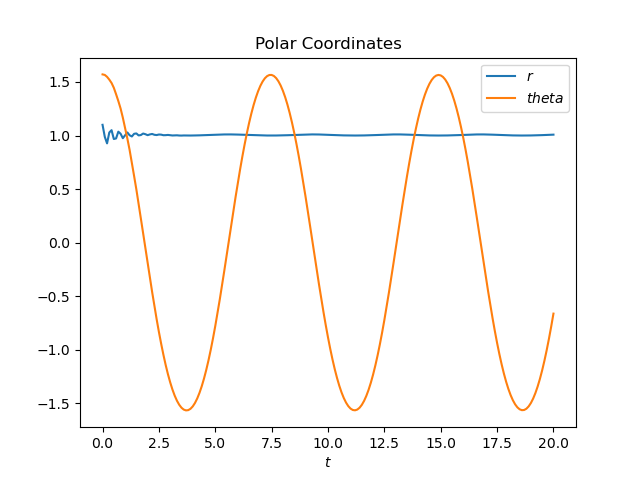
\includegraphics[width=\textwidth]{../Plots/RK4/rk4_h=0.1_k=300_c}
\caption{RK4 $h=0.1$ $k=300$}
\label{rk4_h=0.1_k=300_c}
\end{minipage}
\end{figure}

\section*{Testing Implicit Methods}

Opposite to the case of explicit methods, for linear problems implicit methods count with an extensive stability region which doesn’t make their stability dependent on the value of the step $k$.
The problem was simulated using Implicit Euler, BDF2 with Fixed Point as corrector and BDFk with Newton as corrector for $k$ between $1$ and $4$. All the following experiments take as initial value $y_0 = [1.1, 0, 0, 0]$ and have $[0, 20]$ for time domain.
It is interesting to see how the oscillation of the spring decays for implicit methods. This decay can be attenuated by reducing the step size or accelerated by increasing the value of the spring constant.

\begin{figure}[h]
\centering
\begin{minipage}[b]{0.45\textwidth}
\centering
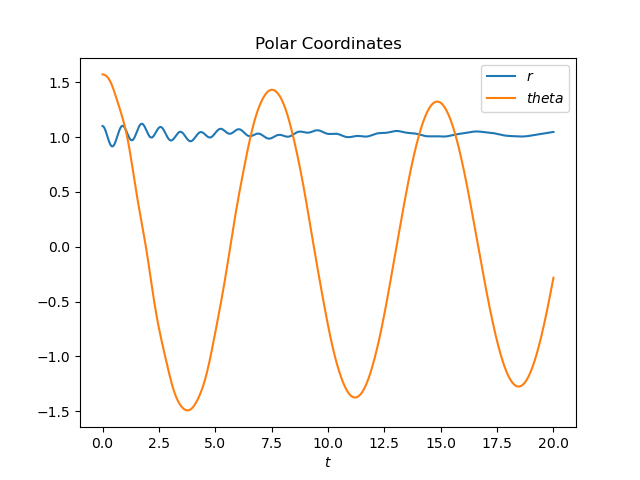
\includegraphics[width=\textwidth]{../Plots/ImpEuler/imp_euler_h=0.01_k=50_c}
\caption{Implicit Euler $h=0.01$ $k=50$}
\label{imp_euler_h=0.01_k=50_c}
\end{minipage}
\end{figure}

\begin{figure}[h]
\centering
\begin{minipage}[b]{0.45\textwidth}
\centering
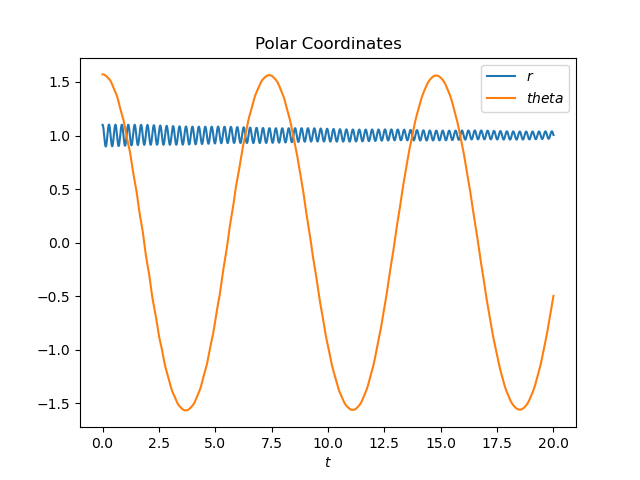
\includegraphics[width=\textwidth]{../Plots/BDF2/bdf2_h=0.01_k=500_c}
\caption{BDF2-Fixed Point $h=0.001$ $k=500$}
\label{exp_euler_k=50_h=0.001_c}
\end{minipage}
\hfill
\begin{minipage}[b]{0.45\textwidth}
\centering
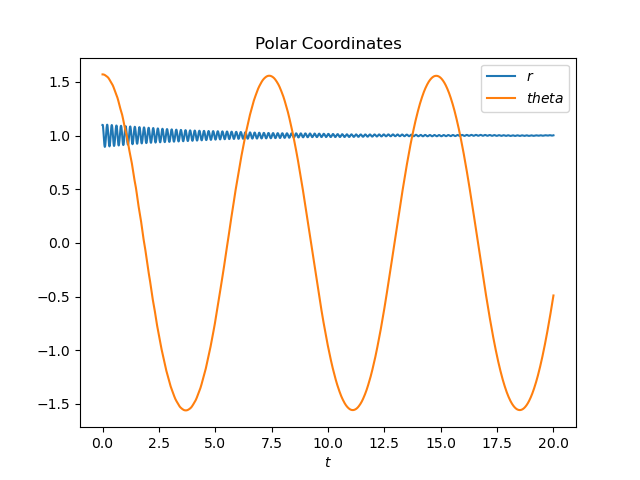
\includegraphics[width=\textwidth]{../Plots/BDF2/bdf2_h=0.01_k=1000_c}
\caption{BDF2-Fixed Point $h=0.01$ $k=1000$}
\label{bdf2_h=00.1_k=1000_c}
\end{minipage}
\end{figure}

The method BDFk with Newton presents a decay in the spring oscillation as the other methods do.
However, it also shows decay of the pendulum oscillation which cannot be observed in the other implicit methods.
To better observe this decay (Figure \ref{bdf2_h=0.01_h=100_tf=100} and Figure \ref{bdf4_h=0.01_h=100_tf=100.png}) the domain is increased to $[0, 100]$.

\begin{figure}[h]
\centering
\begin{minipage}[b]{0.45\textwidth}
\centering
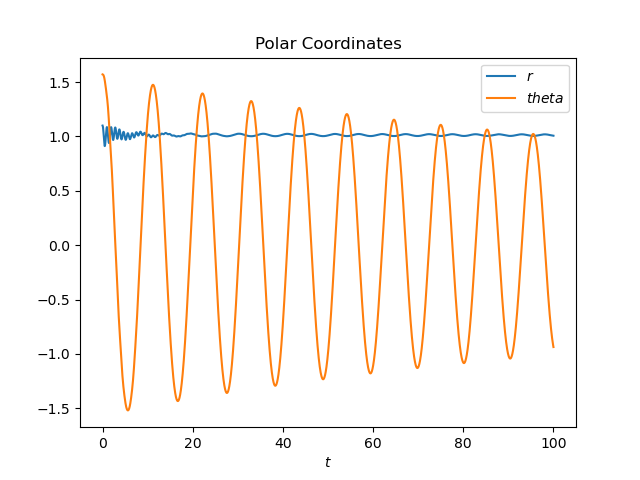
\includegraphics[width=\textwidth]{../Plots/BDFk/bdf2_h=0.01_h=100_tf=100}
\caption{BDF2-Newton $h=0.01$ $k=100$}
\label{bdf2_h=0.01_h=100_tf=100}
\end{minipage}
\hfill
\begin{minipage}[b]{0.45\textwidth}
\centering
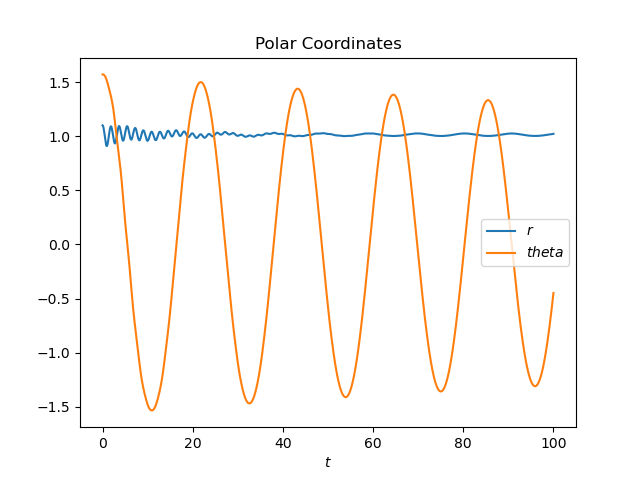
\includegraphics[width=\textwidth]{../Plots/BDFk/bdf4_h=0.01_h=100_tf=100}
\caption{BDF4-Newton $h=0.01$ $k=100$}
\label{bdf4_h=0.01_h=100_tf=100.png}
\end{minipage}
\end{figure}

It is interesting to see how the relation between the speed of decay of the spring oscillation in inversely proportional to the size of the stability region of the methods tested.


\section*{Testing CVODE}
\subsection*{A first test series}

In the first specific test of CVODE we solve our toy problem for increasing $k$. Here we switch between the BDF and Adam-Moultons discretisation method. We also vary the \pyth{maxorder} parameter for both methods.
A higher $k$ reflects a problem which is more stiff. As a stiff problem requires smaller steps the number of steps \pyth{nsteps} increases as $k$ increases which  can be seen in figure \ref{pl:nsteps1}. As the number of function evaluations per stepsize \pyth{nfcns/nsteps} hovers slightly above 1 for all methods (c.f.\ figure \ref{pl:nfcns_nsteps1}) the number of function evaluations increase analogously to \pyth{nsteps} with $k$ as can be seen in figure \ref{pl:nfcns1}. There is however a difference in how many steps each method needs. The BDF-method requires in general more steps than the Adams-Moulton method. And the general trend is that the number of steps increases as \pyth{maxord} is reduced. 

\begin{figure}[h]
\centering
\begin{minipage}[b]{0.45\textwidth}
\centering
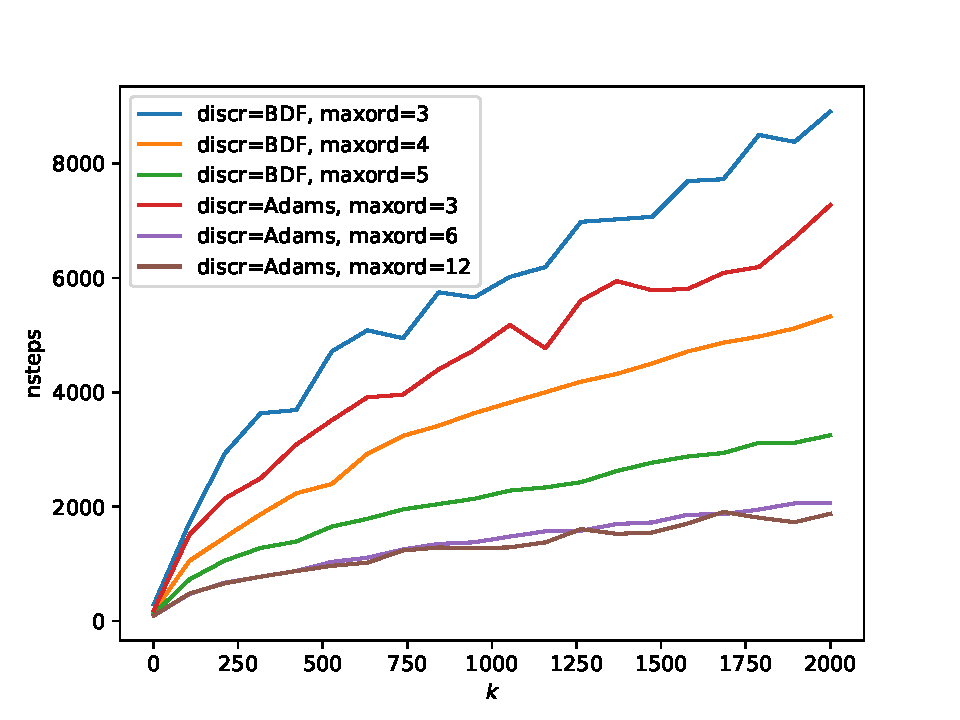
\includegraphics[width=\textwidth]{../Plots/Task4/Figure_200}
\caption{\pyth{nsteps} in relation to the parameter $k$.}
\label{pl:nsteps1}
\end{minipage}
\hfill
\begin{minipage}[b]{0.45\textwidth}
\centering
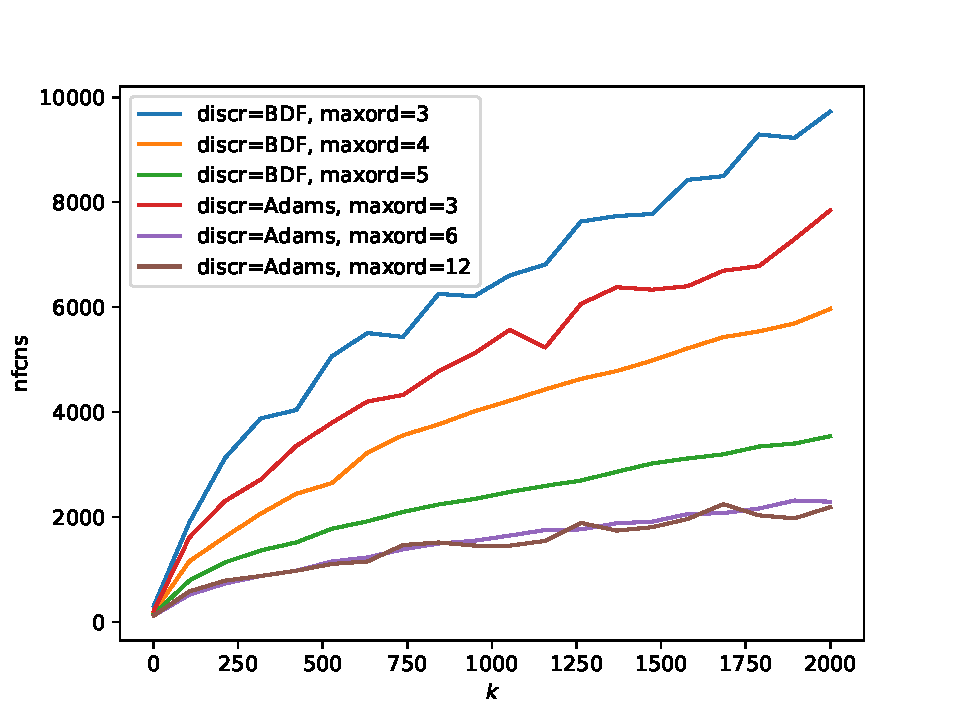
\includegraphics[width=\textwidth]{../Plots/Task4/Figure_201}
\caption{\pyth{nfuncs} in relation to the parameter $k$.}
\label{pl:nfcns1}
\end{minipage}
\end{figure}

From figure \ref{pl:njacs_nsteps1} it can be seen that the number of jacobian evaluations stays roughly constant and happens roughly every 5th step. The number \pyth{nerrfails/steps} stays roughly constant in dependence of $k$ though the general tendency is that it is smaller the lower \pyth{maxord} is set. This makes sense because a lower \pyth{maxord} means there are fewer possibilities for the method order and hence fewer changes of order. In figure \ref{pl:stability1} we see a difference in how much the methods obey the principles of energy conservation. One can see that for growing $k$ the result tends to be further away from physical reality. Once again the methods with higher \pyth{maxord} do better with the exception of the BDF method where for some reason a \pyth{maxord} of 4 performs best.


\begin{figure}[h]
\centering
\begin{minipage}[b]{0.45\textwidth}
\centering
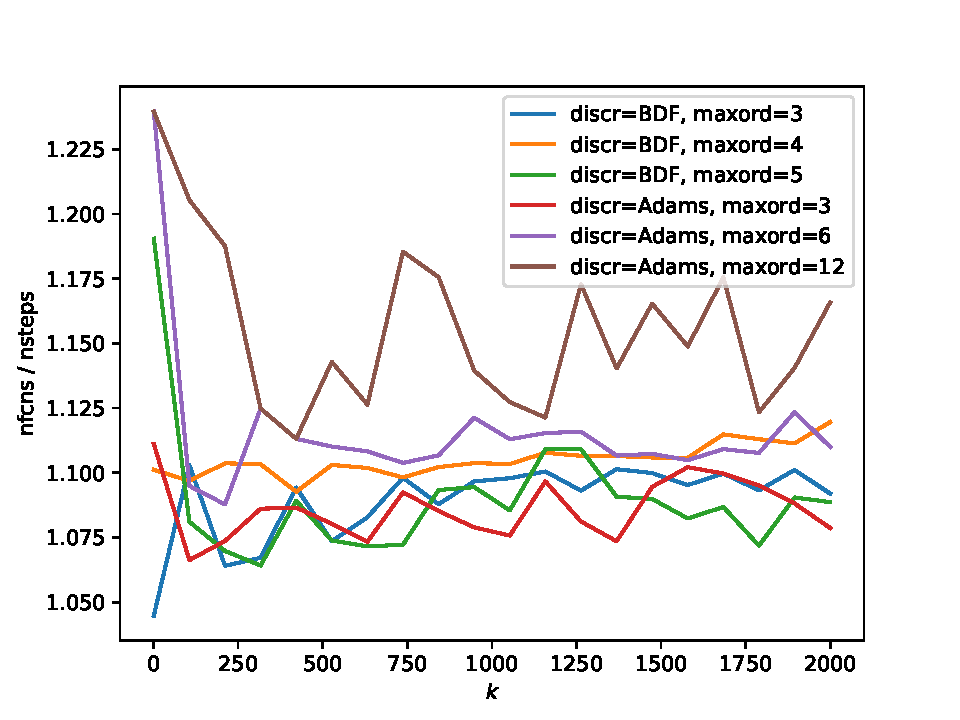
\includegraphics[width=\textwidth]{../Plots/Task4/Figure_210}
\caption{\pyth{nfcns/nsteps} in relation to the parameter $k$.}
\label{pl:nfcns_nsteps1}
\end{minipage}
\hfill
\begin{minipage}[b]{0.45\textwidth}
\centering
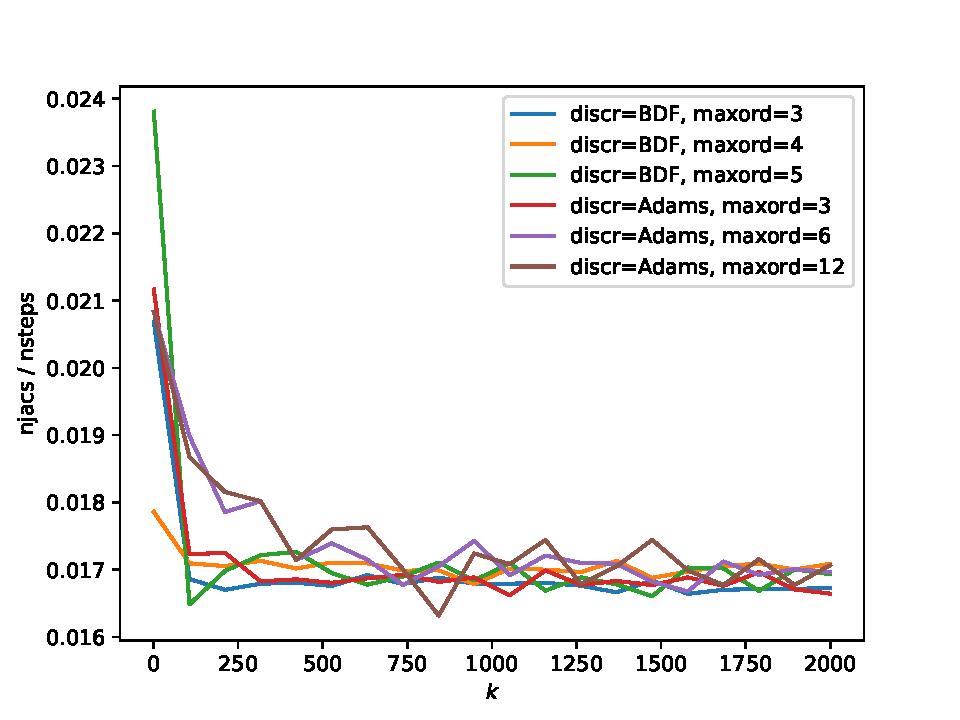
\includegraphics[width=\textwidth]{../Plots/Task4/Figure_211}
\caption{\pyth{njacs/nsteps} in relation to the parameter $k$.}
\label{pl:njacs_nsteps1}
\end{minipage}
\end{figure}


\begin{figure}[h]
\centering
\begin{minipage}[b]{0.45\textwidth}
\centering
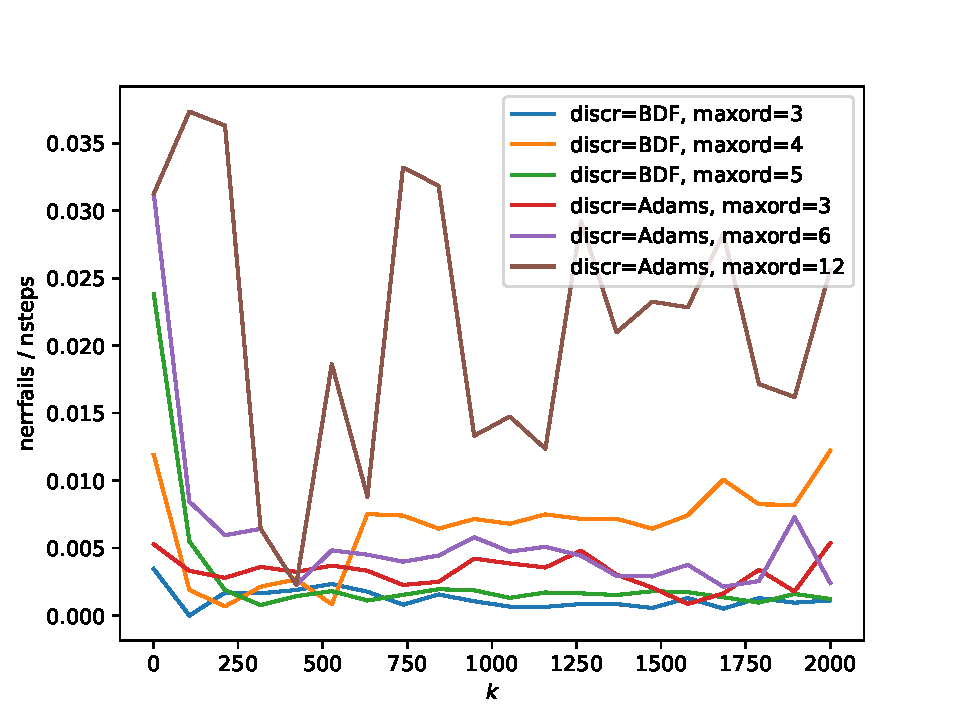
\includegraphics[width=\textwidth]{../Plots/Task4/Figure_212}
\caption{\pyth{nerrfails/nsteps} in relation to the parameter $k$.}
\label{pl:nerrfails_nsteps1}
\end{minipage}
\hfill
\begin{minipage}[b]{0.45\textwidth}
\centering
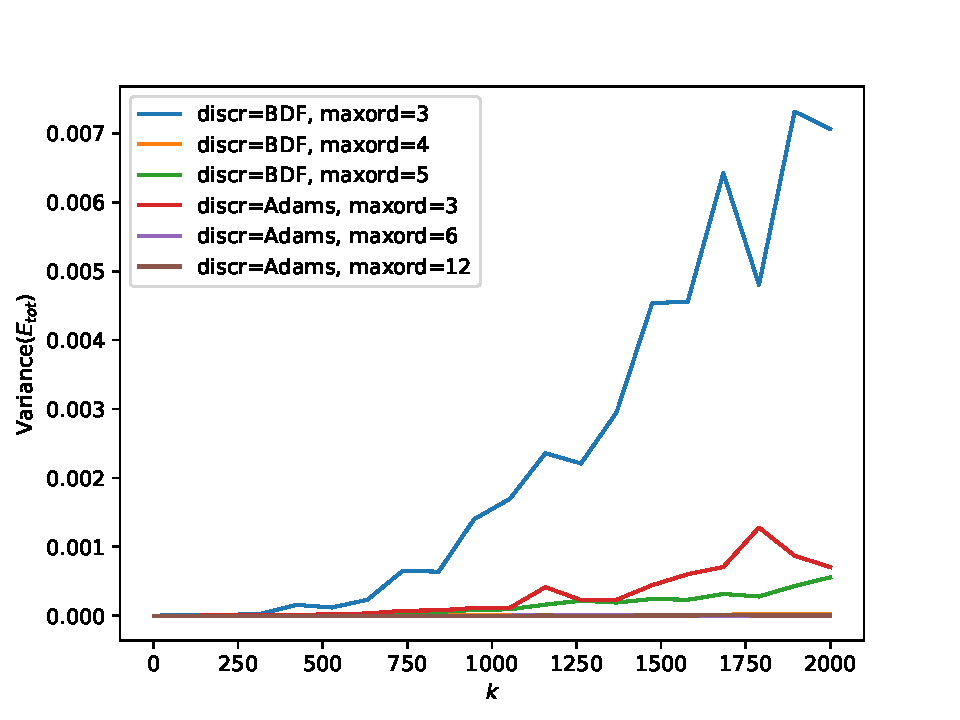
\includegraphics[width=\textwidth]{../Plots/Task4/Figure_204}
\caption{instability index in relation to the parameter $k$.}
\label{pl:stability1}
\end{minipage}
\end{figure}

This test confirms once again that a stiffer Problem needs more function evaluations in CVODE.
Perhaps surprisingly the Adams-Moulton-method seems to perform better on this problem.
This experiment also highlights that a lower \pyth{maxord} parameter tends to be more computationally expensive though it reduces the number of error test failures \pyth{nerrfails}.

\subsection*{Testing the parameter rtol}
We now test the influence of the parameter \pyth{rtol} on the methods BDF and Adams-Moulton. For this we set $k=10^3$ and keep all other parameters on their default values. The results can be seen in figures \ref{pl:nsteps2} to \ref{pl:stability2}. We note that as \pyth{rtol} increases the number of steps decreases (c.f.\ figure \ref{pl:nsteps2}). If one compares figures the instability index for $k\approx10^3$ in figure \ref{pl:stability1} with the instability index in figure \ref{pl:stability2} one sees that changing the \pyth{rtol} parameter from the default makes the result significantly worse in terms of energy conservation.

\begin{figure}[h]
\centering
\begin{minipage}[b]{0.45\textwidth}
\centering
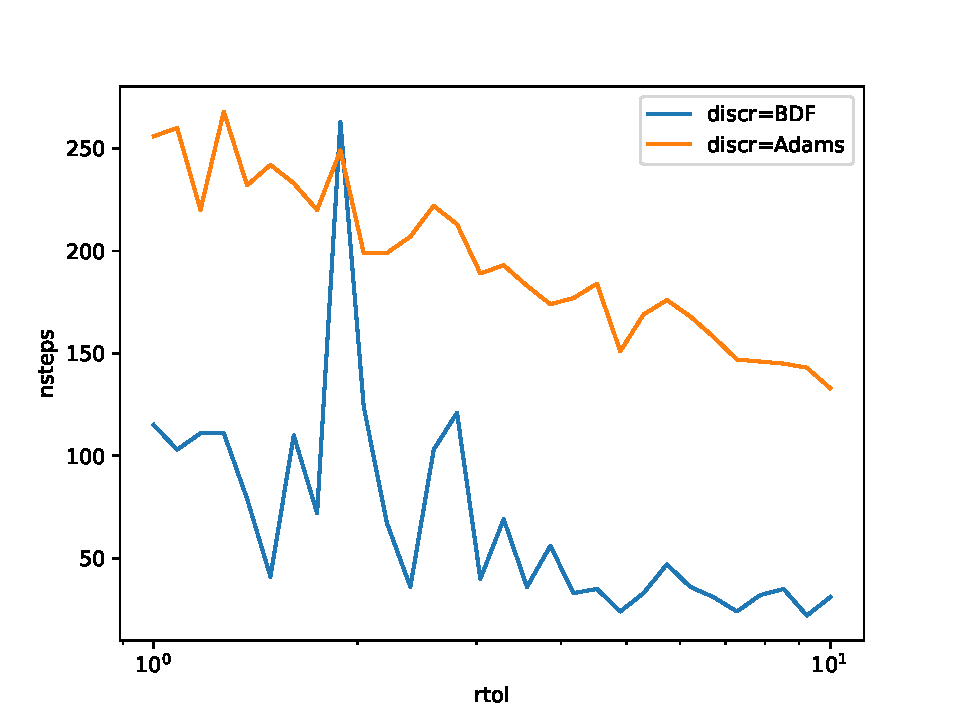
\includegraphics[width=\textwidth]{../Plots/Task4/Figure_300}
\caption{\pyth{nsteps} in relation to the parameter \pyth{rtol}.}
\label{pl:nsteps2}
\end{minipage}
\hfill
\begin{minipage}[b]{0.45\textwidth}
\centering
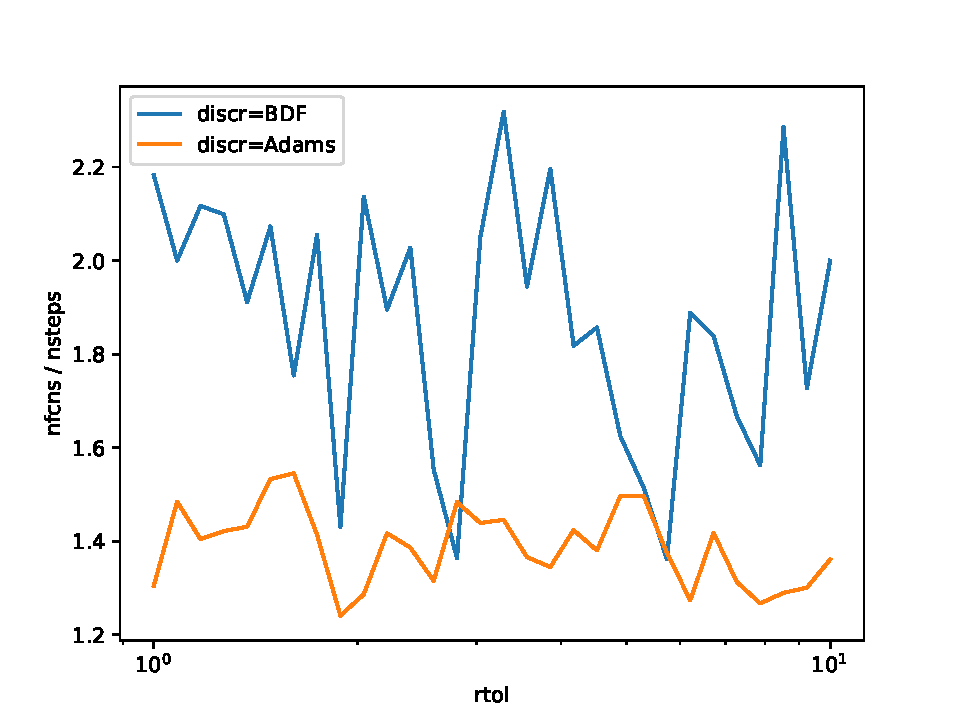
\includegraphics[width=\textwidth]{../Plots/Task4/Figure_310}
\caption{\pyth{nfcns/nsteps} in relation to the parameter \pyth{rtol}.}
\label{pl:nfcns_nsteps2}
\end{minipage}
\end{figure}


\begin{figure}[h]
\centering
\begin{minipage}[b]{0.45\textwidth}
\centering
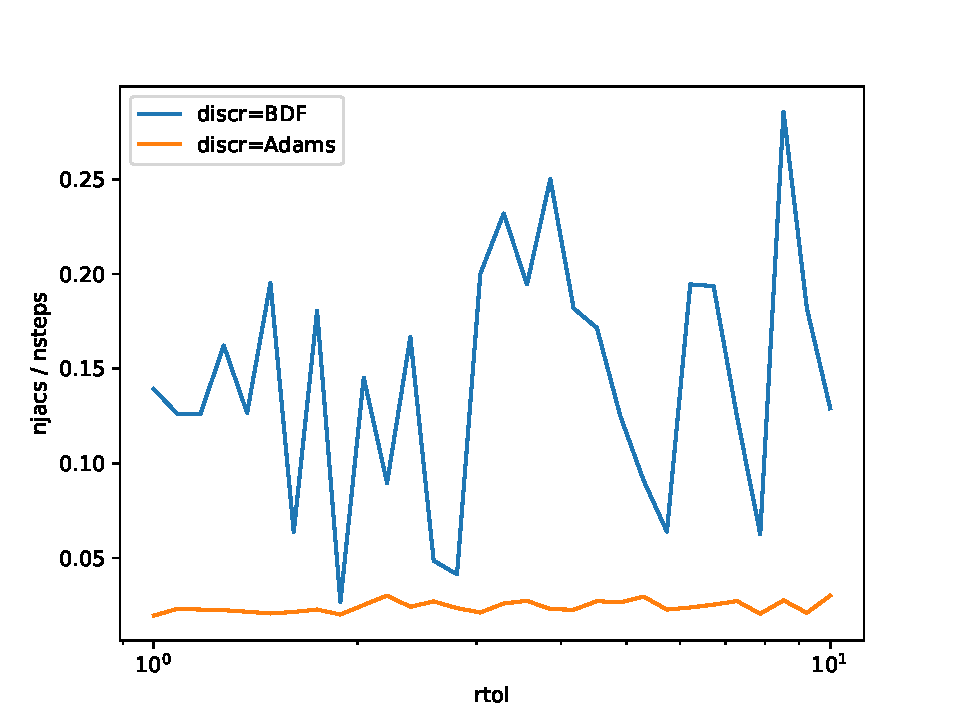
\includegraphics[width=\textwidth]{../Plots/Task4/Figure_311}
\caption{\pyth{njacs/nsteps} in relation to the parameter \pyth{rtol}.}
\label{pl:njacs_nsteps2}
\end{minipage}
\hfill
\begin{minipage}[b]{0.45\textwidth}
\centering
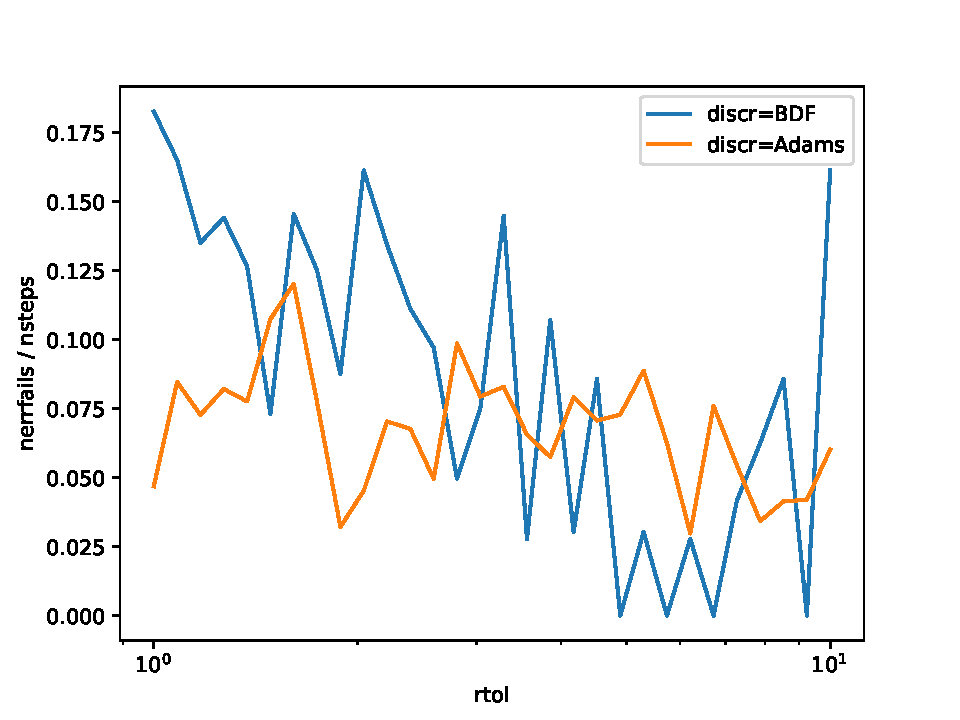
\includegraphics[width=\textwidth]{../Plots/Task4/Figure_312}
\caption{\pyth{nerrfails/nsteps} in relation to the parameter \pyth{rtol}.}
\label{pl:nerrfails_nsteps2}
\end{minipage}
\end{figure}


\begin{figure}[h]
\centering
\begin{minipage}[b]{0.45\textwidth}
\centering
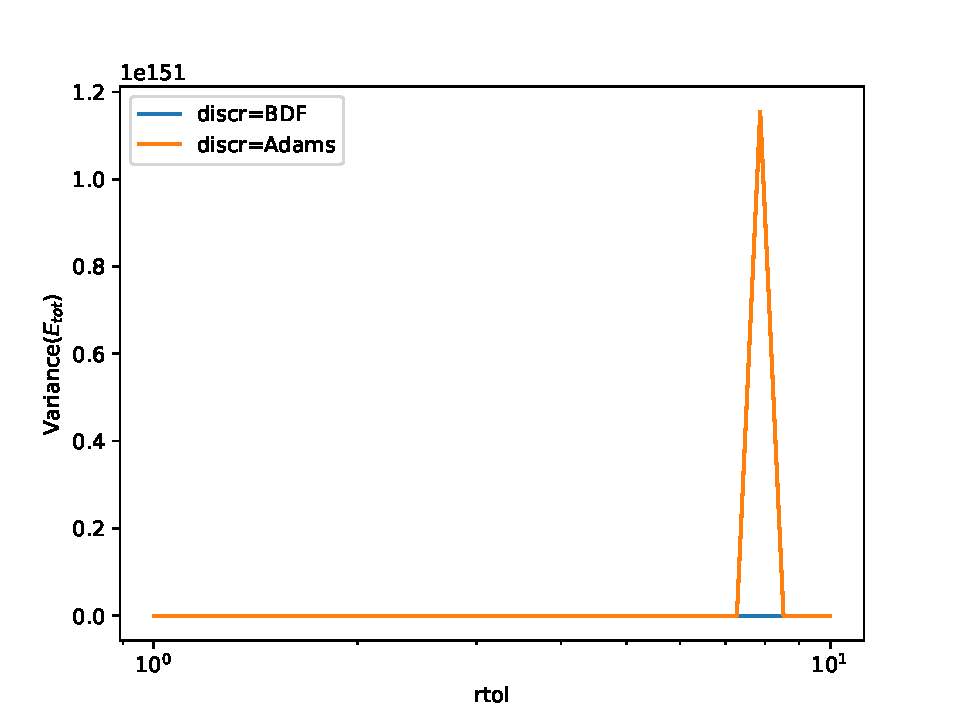
\includegraphics[width=\textwidth]{../Plots/Task4/Figure_304}
\caption{instability index in relation to the parameter \pyth{rtol}.}
\label{pl:stability2}
\end{minipage}
\end{figure}

\subsection*{Testing the parameter atol}

If we test the \pyth{atol} parameter on the Adams and Newton method analogously to the test of the \pyth{rtol} parameter we once again get an instability index that is significantly above the value for the method in which we did not specify this value as can be seen in Figure \ref{pl:stability3}. In either case we observe that fixing the tolerance seems to come at the cost of energy conversation as is dramatically visualised in Figures \ref{pl:energy2} and \ref{pl:energy3}.


\begin{figure}[h]
\centering
\begin{minipage}[b]{0.45\textwidth}
\centering
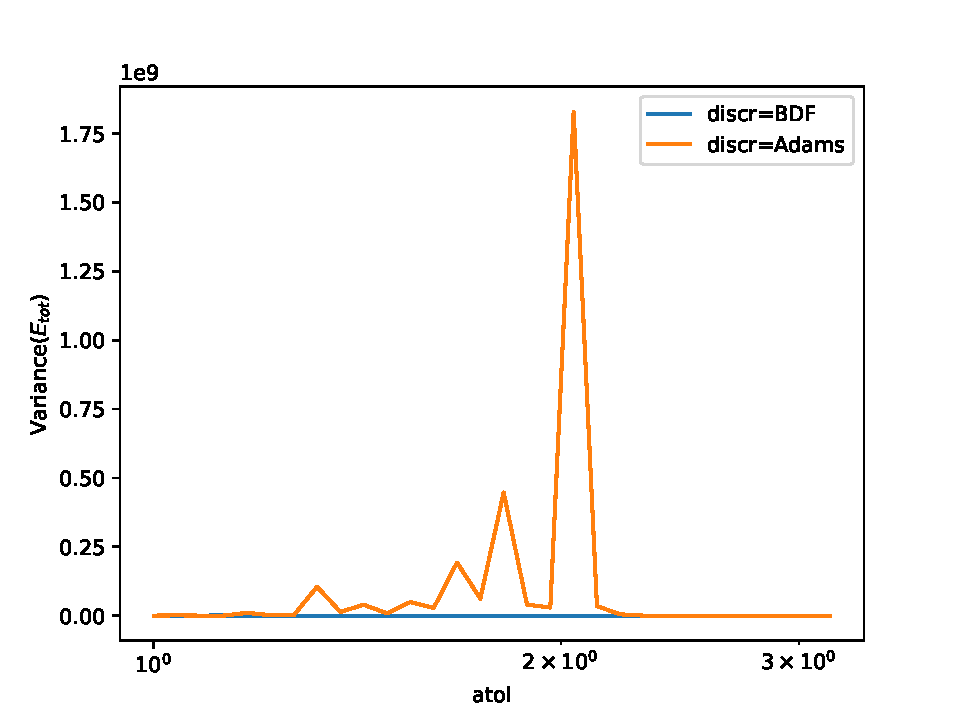
\includegraphics[width=\textwidth]{../Plots/Task4/Figure_404}
\caption{instability index in relation to the parameter \pyth{atol}.}
\label{pl:stability3}
\end{minipage}
\end{figure}

\begin{figure}[h]
\centering
\begin{minipage}[b]{0.45\textwidth}
\centering
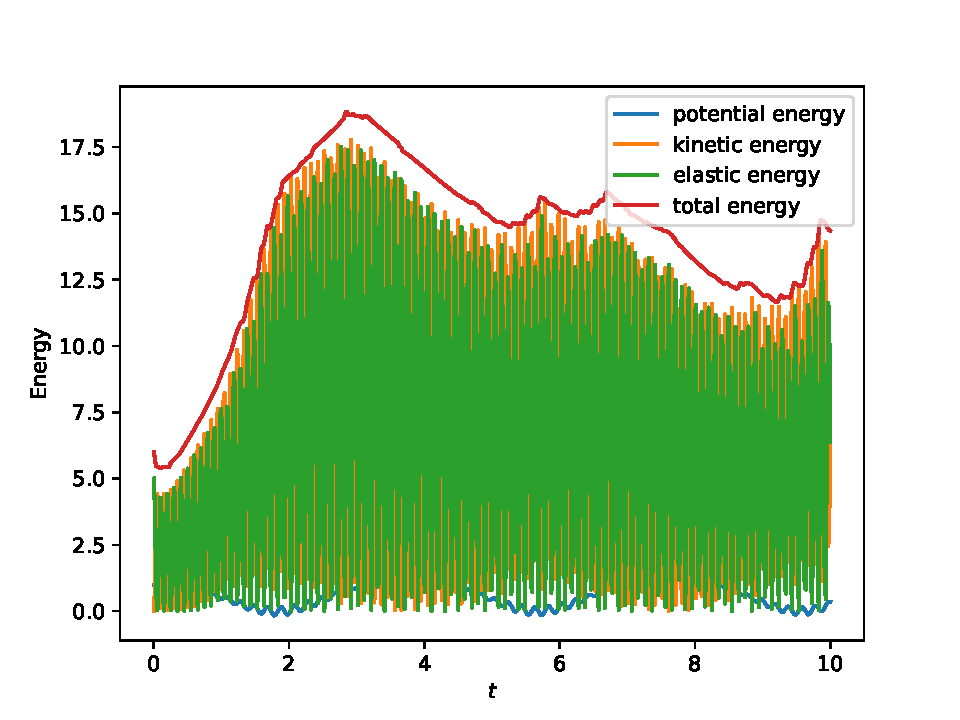
\includegraphics[width=\textwidth]{../Plots/Task4/Figure_450}
\caption{Energy plot for $k=10^3$ with \pyth{atol=1E-2}.}
\label{pl:energy2}
\end{minipage}
\hfill
\begin{minipage}[b]{0.45\textwidth}
\centering
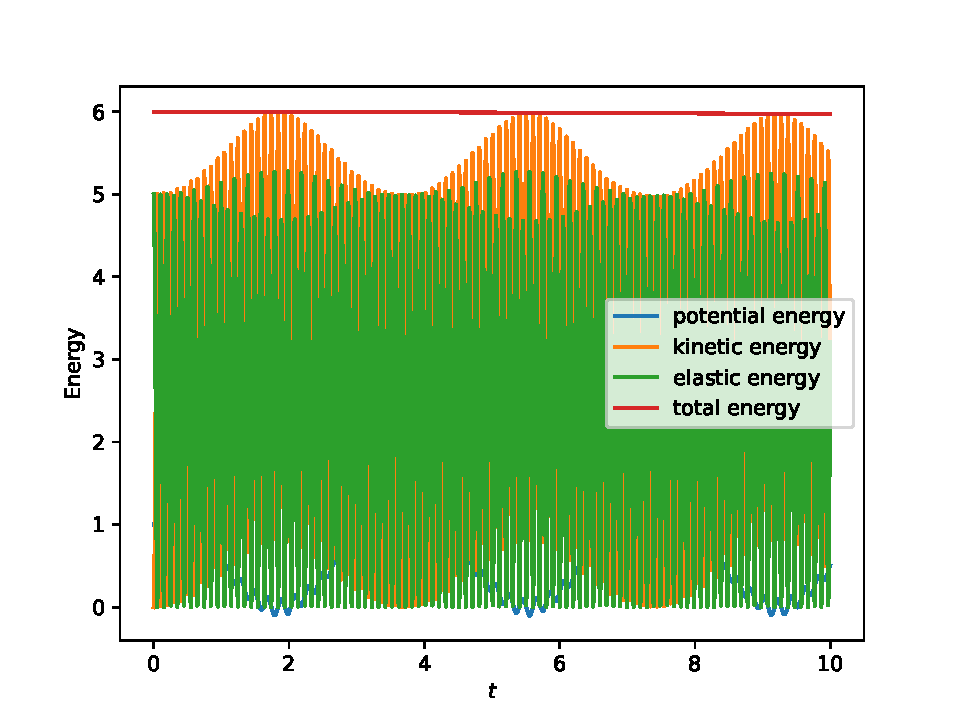
\includegraphics[width=\textwidth]{../Plots/Task4/Figure_451}
\caption{Energy plot for $k=10^3$.}
\label{pl:energy3}
\end{minipage}
\end{figure}

All in all we see that none of the (admittedly crude) tweaking of the parameters improved the performance of CVODE. To the contrary, most changes worsened the performance. The choice of the discretisation method on the other hand did make a big difference and the performance for solving the toy problem could be improved by switching from the default BDF method.


\chapter*{Project 2}

\newpage


% here come some stability regions

\begin{figure}[h]
\centering
\begin{minipage}[b]{0.45\textwidth}
\centering
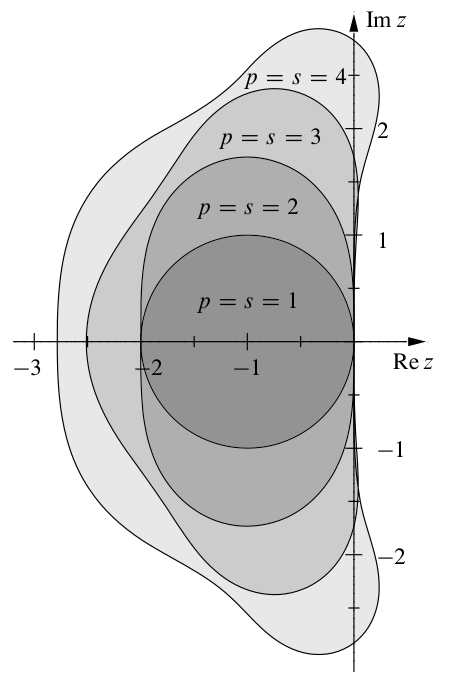
\includegraphics[width=\textwidth]{../Drawings/Runge_Kutter_stability_regions}
\caption{Stability regions of the Runge-Kutta-methods, taken from \cite{Stab_RK}[p.238]}
\end{minipage}
\end{figure}

\begin{figure}[h]
\centering
\begin{minipage}[b]{0.45\textwidth}
\centering
\hspace*{-1cm}
\scalebox{0.42}{
\input{../Drawings/Stability_region_for_BDF1.pdf_tex}
}
\caption{Stability region for BDF1, taken from \cite{Stab_BDF}}
\end{minipage}
\hfill
\begin{minipage}[b]{0.45\textwidth}
\centering
\hspace*{-1cm}
\scalebox{0.42}{
\input{../Drawings/Stability_region_for_BDF2.pdf_tex}
}
\caption{Stability region for BDF2, taken from \cite{Stab_BDF}}
\end{minipage}
\end{figure}

\begin{figure}[h]
\centering
\begin{minipage}[b]{0.45\textwidth}
\centering
\hspace*{-1cm}
\scalebox{0.42}{
\input{../Drawings/Stability_region_for_BDF3.pdf_tex}
}
\caption{Stability region for BDF3, taken from \cite{Stab_BDF}}
\end{minipage}
\hfill
\begin{minipage}[b]{0.45\textwidth}
\centering
\hspace*{-1cm}
\scalebox{0.42}{
\input{../Drawings/Stability_region_for_BDF4.pdf_tex}
}
\caption{Stability region for BDF4, taken from \cite{Stab_BDF}}
\end{minipage}
\end{figure}

\begin{figure}[h]
\centering
\begin{minipage}[b]{0.45\textwidth}
\centering
\hspace*{-1cm}
\scalebox{0.42}{
\input{../Drawings/Stability_region_for_BDF5.pdf_tex}
}
\caption{Stability region for BDF5, taken from \cite{Stab_BDF}}
\end{minipage}
\hfill
\begin{minipage}[b]{0.45\textwidth}
\centering
\hspace*{-1cm}
\scalebox{0.42}{
\input{../Drawings/Stability_region_for_BDF6.pdf_tex}
}
\caption{Stability region for BDF6, taken from \cite{Stab_BDF}}
\end{minipage}
\end{figure}

%\nocite{*}
\printbibliography

\end{document}
